\chapter{Sprint 4: Alerts Management and Energy Consumption Monitoring}

\section{Introduction}

Sprint 4 represents a critical advancement in the TelecomOps platform, focusing on two essential subsystems: the Alerts Management System and the Energy Consumption Monitoring System. These implementations address critical operational requirements for proactive network management and energy efficiency optimization.

The Alerts Management System provides real-time notification capabilities for network anomalies, equipment failures, and maintenance requirements with status transitions from active to acknowledged to resolved. The Energy Consumption Monitoring System enables comprehensive tracking and analysis of power consumption across network sites with automatic cost calculation, visual analytics, and threshold-based alerting.

Both systems integrate seamlessly with existing platform architecture, leveraging Supabase real-time subscriptions, PostgreSQL with Row-Level Security, and Next.js 14 capabilities. This sprint delivers eight user stories encompassing automated alert generation, real-time notifications, energy recording, trend visualization, and consumption analytics.

\section{Sprint Backlog}

\begin{table}[htbp]
\centering
\caption{Sprint 4 Backlog - User Stories}
\small
\begin{tabular}{|p{0.8cm}|p{9cm}|p{1.8cm}|}
\hline
\textbf{ID} & \textbf{User Story} & \textbf{Priority} \\
\hline
US-4.1 & As a system, I want to automatically create alerts when equipment faults are detected & Critical \\
\hline
US-4.2 & As a manager, I want to acknowledge critical alerts to track response time & High \\
\hline
US-4.3 & As an engineer, I want to resolve alerts after fixing issues & High \\
\hline
US-4.4 & As a user, I want real-time notifications for critical alerts & Critical \\
\hline
US-4.5 & As a manager, I want to record energy consumption data for each site & High \\
\hline
US-4.6 & As an engineer, I want to view energy consumption trends with charts & Medium \\
\hline
US-4.7 & As a manager, I want to calculate energy costs automatically & High \\
\hline
US-4.8 & As an admin, I want to track consumption per day and identify patterns & Medium \\
\hline
\end{tabular}
\end{table}

\section{Class Diagram}

\begin{figure}[H]
\centering
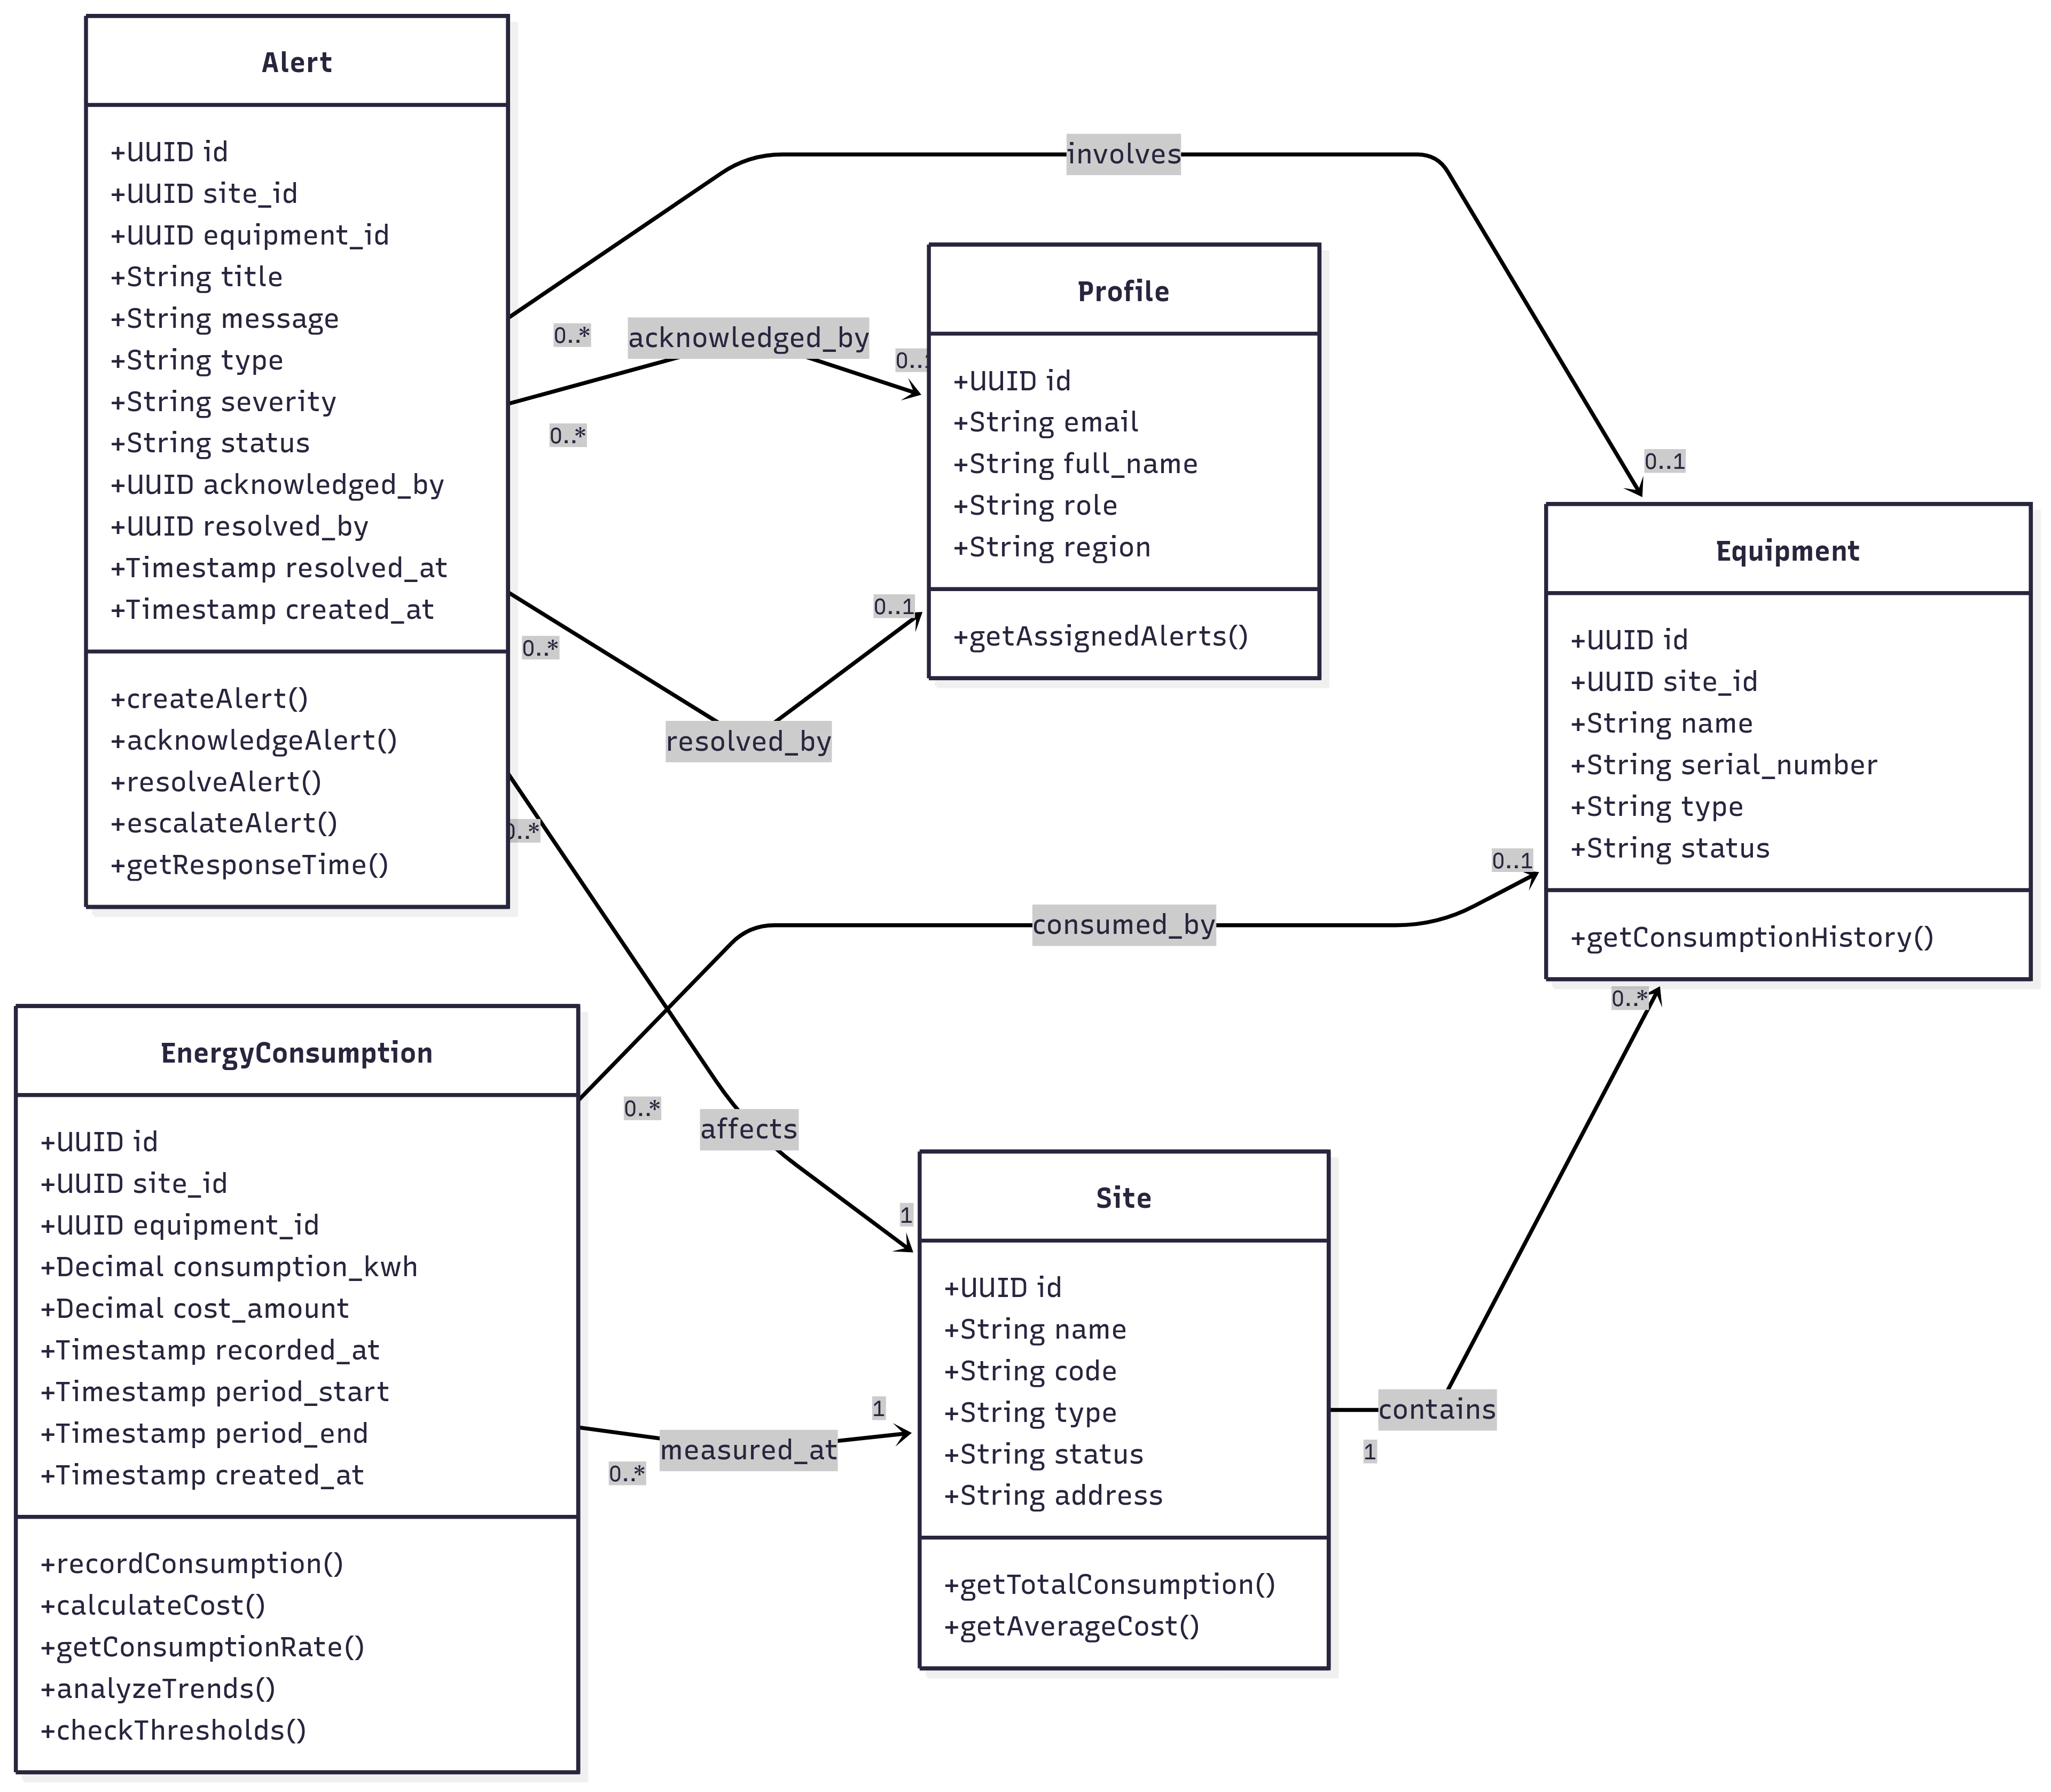
\includegraphics[width=0.7\textwidth]{img/chap_06/class_diagram_sprint4.png}
\caption{Class Diagram - Alert and Energy Consumption Entities}
\end{figure}

The Alert class manages system notifications with attributes for title, message, type, severity, and status. It implements methods for creation, acknowledgment, resolution, and escalation. The EnergyConsumption class captures power usage with consumption in kWh, costs, timestamps, and periods. It supports recording, cost calculation, rate analysis, and threshold validation.

\section{Use Case Diagram}

\begin{figure}[H]
\centering
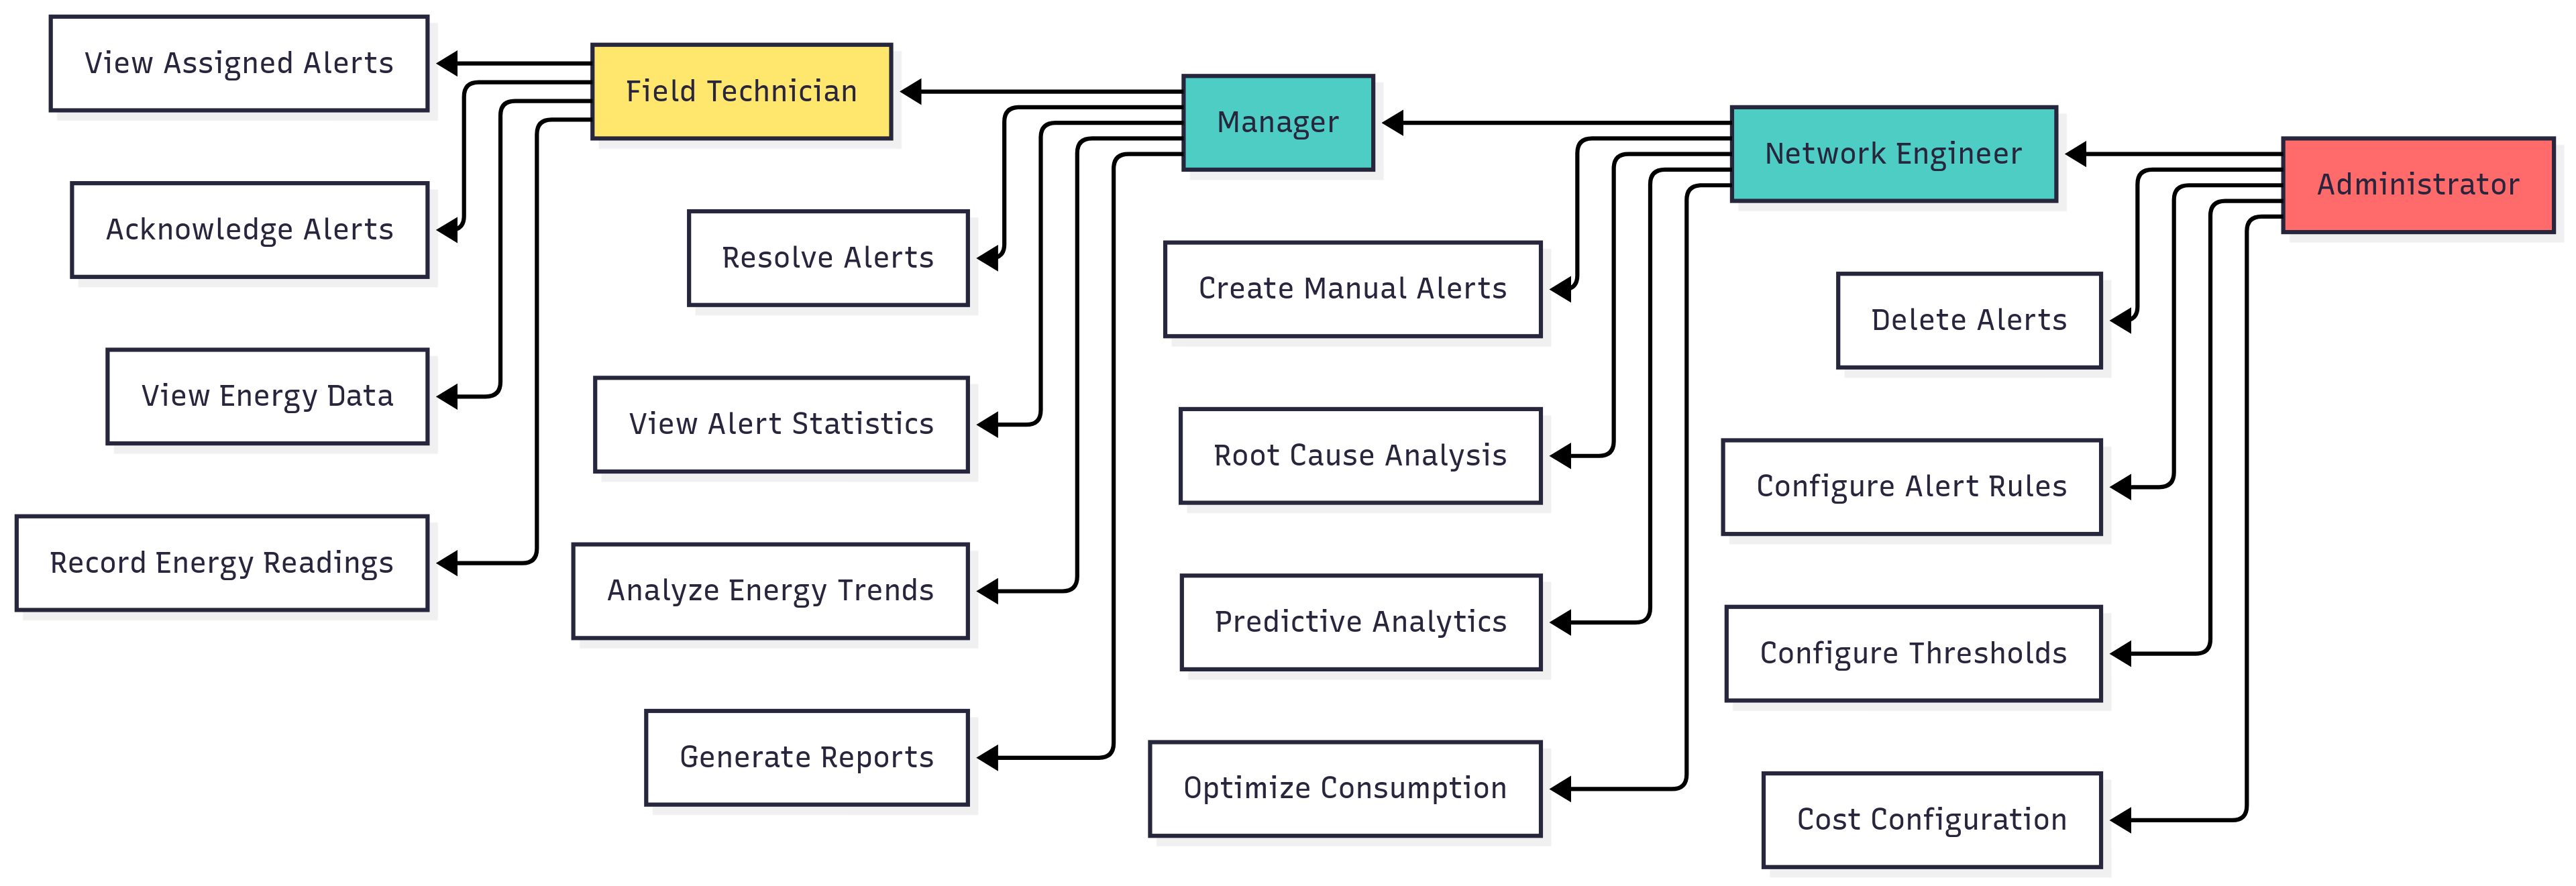
\includegraphics[width=0.7\textwidth]{img/chap_06/usecase_diagram_sprint4.png}
\caption{Use Case Diagram - Role-based Alerts and Energy Management}
\end{figure}

The diagram models role hierarchies: Field Technician has base permissions, Manager extends with alert creation and analysis, Network Engineer adds predictive analytics, and Administrator has complete system control.

\section{Use Case Permissions}

\begin{table}[htbp]
\centering
\caption{Use Case Permissions Matrix}
\small
\begin{tabular}{|p{4.5cm}|c|c|c|c|}
\hline
\textbf{Use Case} & \textbf{Tech} & \textbf{Mgr} & \textbf{Eng} & \textbf{Admin} \\
\hline
View Assigned Alerts & Yes & Yes & Yes & Yes \\
\hline
Acknowledge Alerts & Yes & Yes & Yes & Yes \\
\hline
Resolve Alerts & No & Yes & Yes & Yes \\
\hline
Create Manual Alerts & No & Yes & Yes & Yes \\
\hline
Delete Alerts & No & No & No & Yes \\
\hline
Configure Alert Rules & No & No & No & Yes \\
\hline
View Energy Data & Yes & Yes & Yes & Yes \\
\hline
Record Energy Readings & Yes & Yes & Yes & Yes \\
\hline
Analyze Energy Trends & No & Yes & Yes & Yes \\
\hline
Predictive Analytics & No & No & Yes & Yes \\
\hline
Configure Thresholds & No & No & No & Yes \\
\hline
Generate Reports & No & Yes & Yes & Yes \\
\hline
\end{tabular}
\end{table}

\section{Detailed Use Case: Create Alert}

\begin{table}[htbp]
\centering
\caption{Use Case Description: Create Alert}
\small
\begin{tabular}{|p{3.5cm}|p{10cm}|}
\hline
\textbf{Use Case} & Create System Alert \\
\hline
\textbf{Actors} & Network Engineer, Manager, Administrator \\
\hline
\textbf{Preconditions} & User authenticated with appropriate role. Sites and equipment data available. \\
\hline
\textbf{Main Flow} & 1. User clicks "Create Alert" button, 2. System displays form, 3. User enters title and message, 4. User selects type and severity, 5. User selects site and optional equipment, 6. User submits form, 7. System validates fields, 8. System creates alert with "active" status, 9. System triggers real-time notification, 10. System displays confirmation \\
\hline
\textbf{Alternative Flows} & A1: Validation failure - display errors. A2: Critical alert - send immediate notifications \\
\hline
\textbf{Postconditions} & Alert stored in database. Real-time notification delivered. System log created. \\
\hline
\end{tabular}
\end{table}

\section{Sequence Diagrams}

\begin{figure}[H]
\centering
\begin{minipage}{0.48\textwidth}
\centering
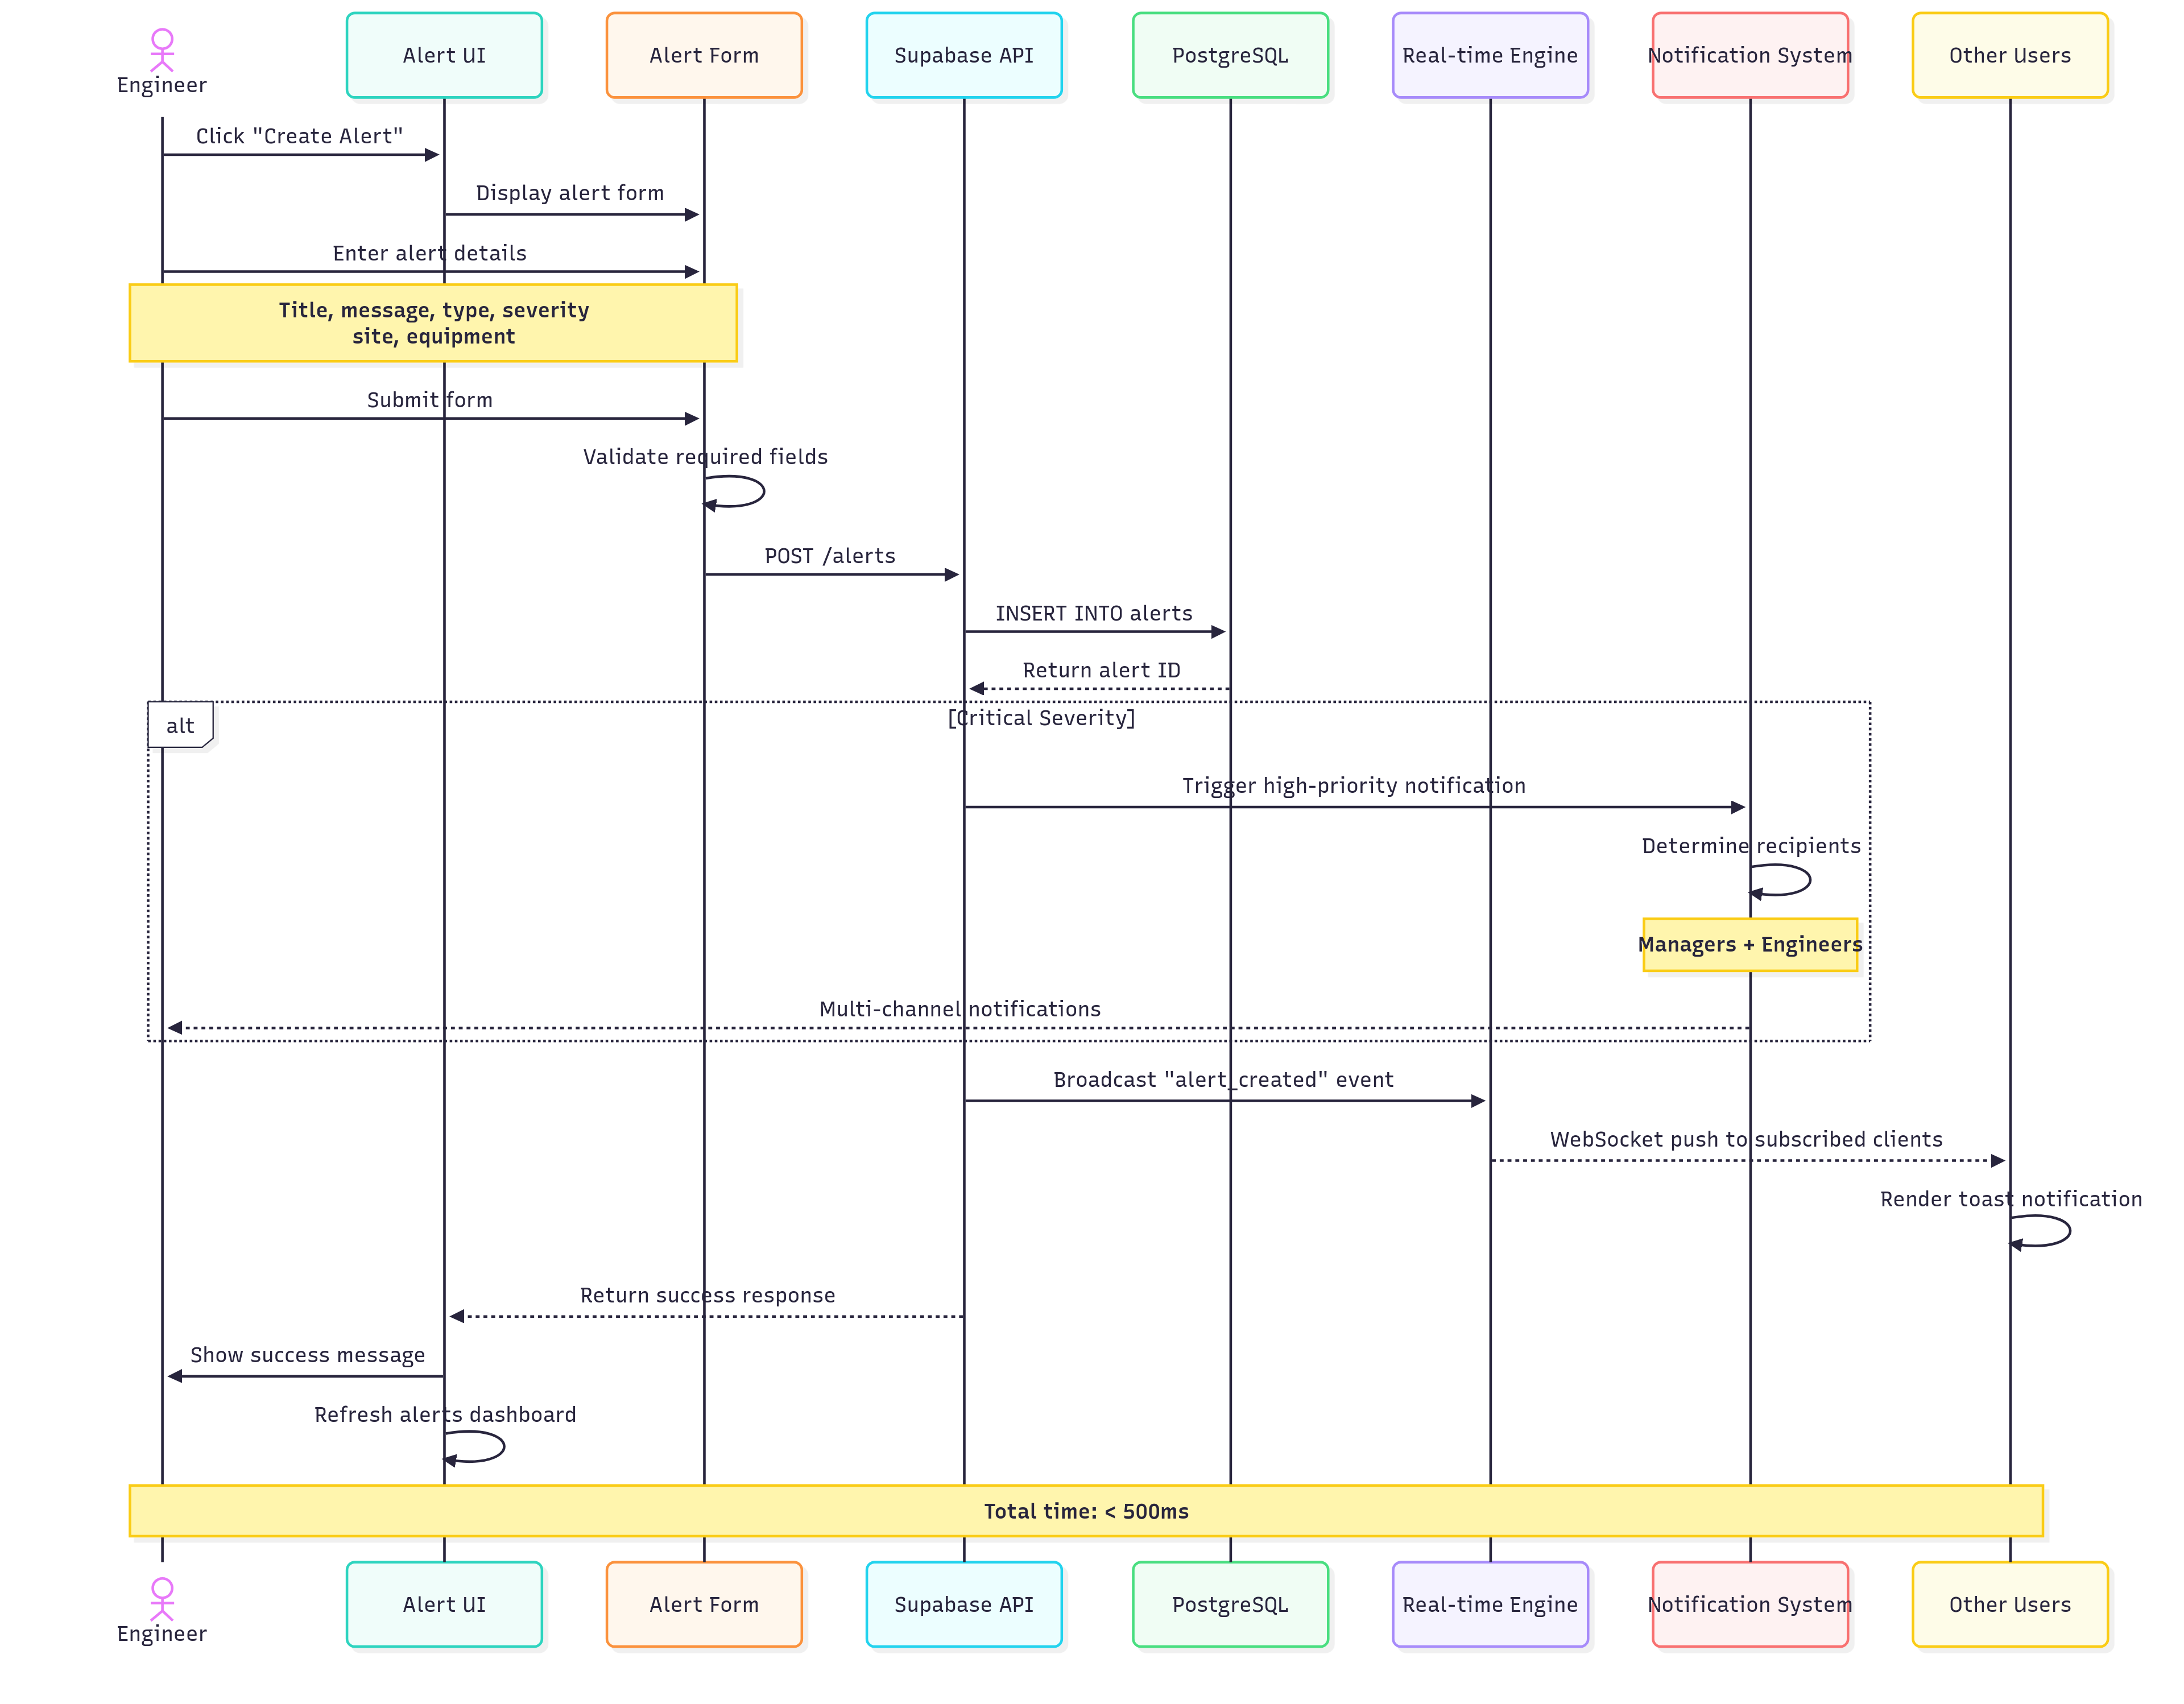
\includegraphics[width=0.95\textwidth]{img/chap_06/sequence_create_alert.png}
\caption{Create Alert Sequence}
\end{minipage}
\hfill
\begin{minipage}{0.48\textwidth}
\centering
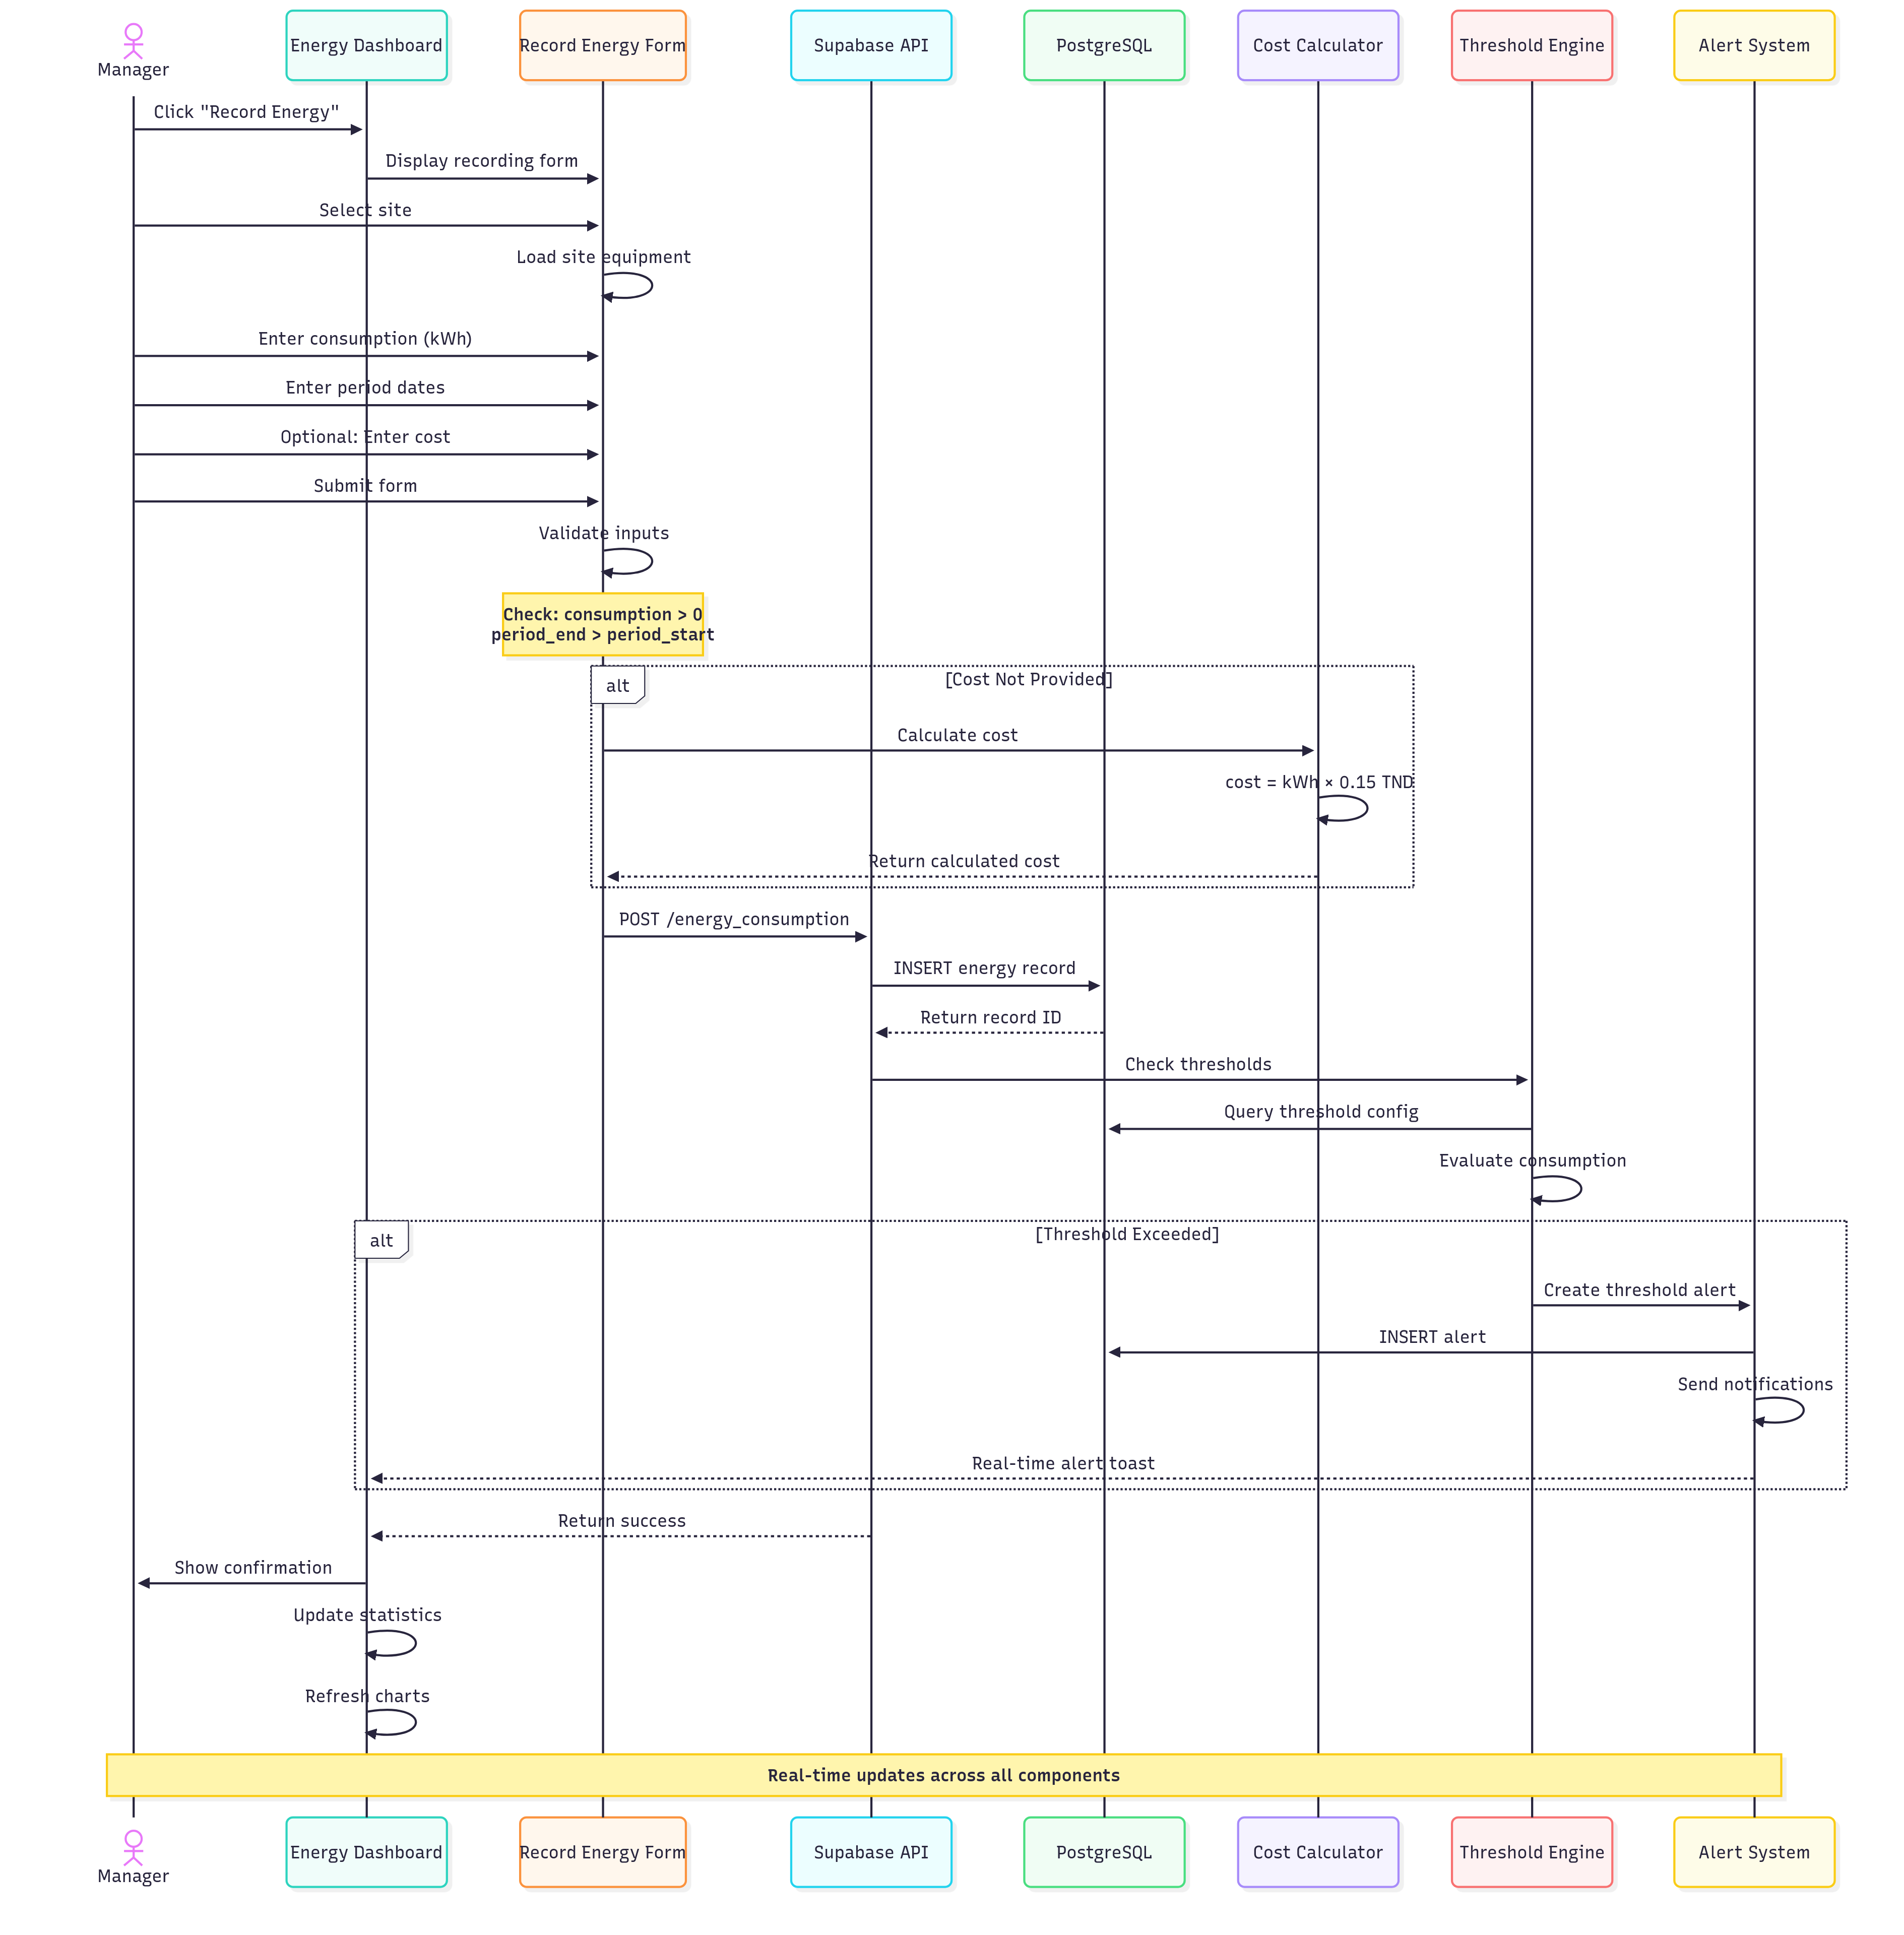
\includegraphics[width=0.95\textwidth]{img/chap_06/sequence_record_energy.png}
\caption{Record Energy Sequence}
\end{minipage}
\end{figure}

The create alert sequence shows: Engineer initiates creation, UI validates and submits to Supabase API, system inserts into PostgreSQL, triggers notifications for critical alerts via Real-time Engine broadcasting WebSocket events to clients. The record energy sequence demonstrates: Manager enters consumption data, Cost Calculator computes cost at 0.15 TND/kWh if not provided, Threshold Engine validates limits and creates alerts if exceeded.

\section{Implementation Screenshots}

\begin{figure}[H]
\centering
\begin{minipage}{0.48\textwidth}
\centering
\fbox{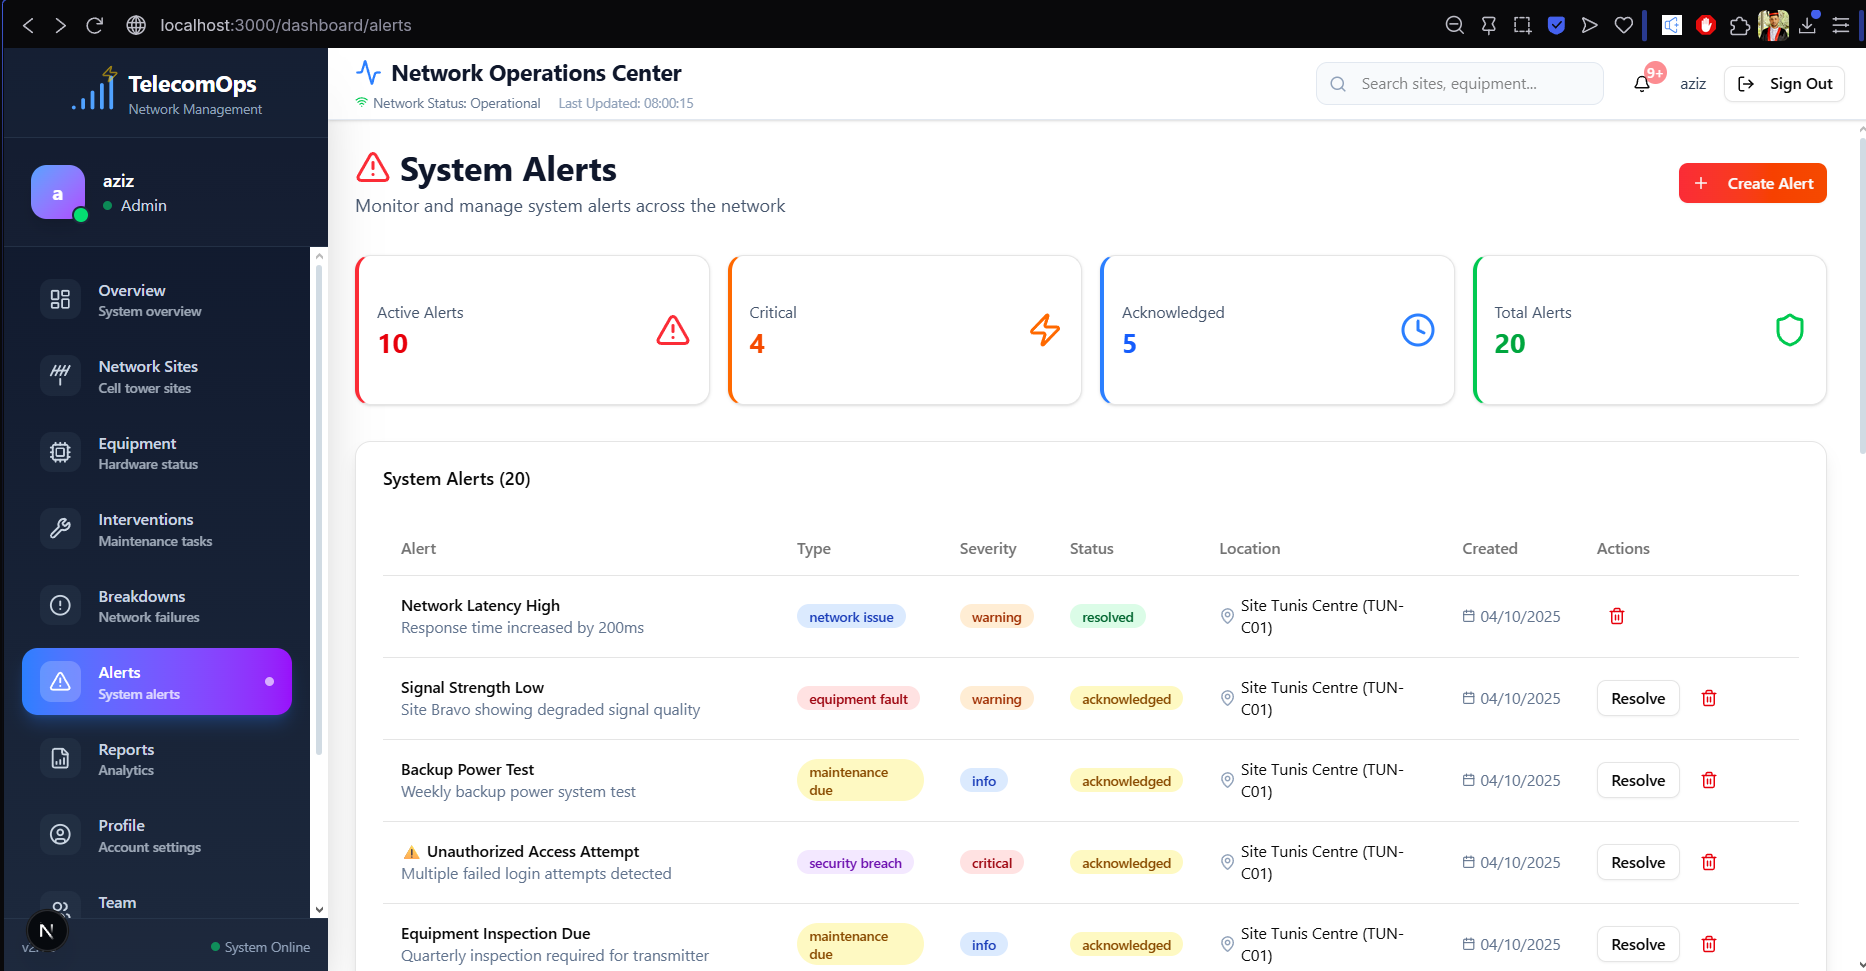
\includegraphics[width=0.95\textwidth]{img/chap_06/screenshot_alerts_dashboard.png}}
\caption{Alerts Dashboard}
\end{minipage}
\hfill
\begin{minipage}{0.48\textwidth}
\centering
\fbox{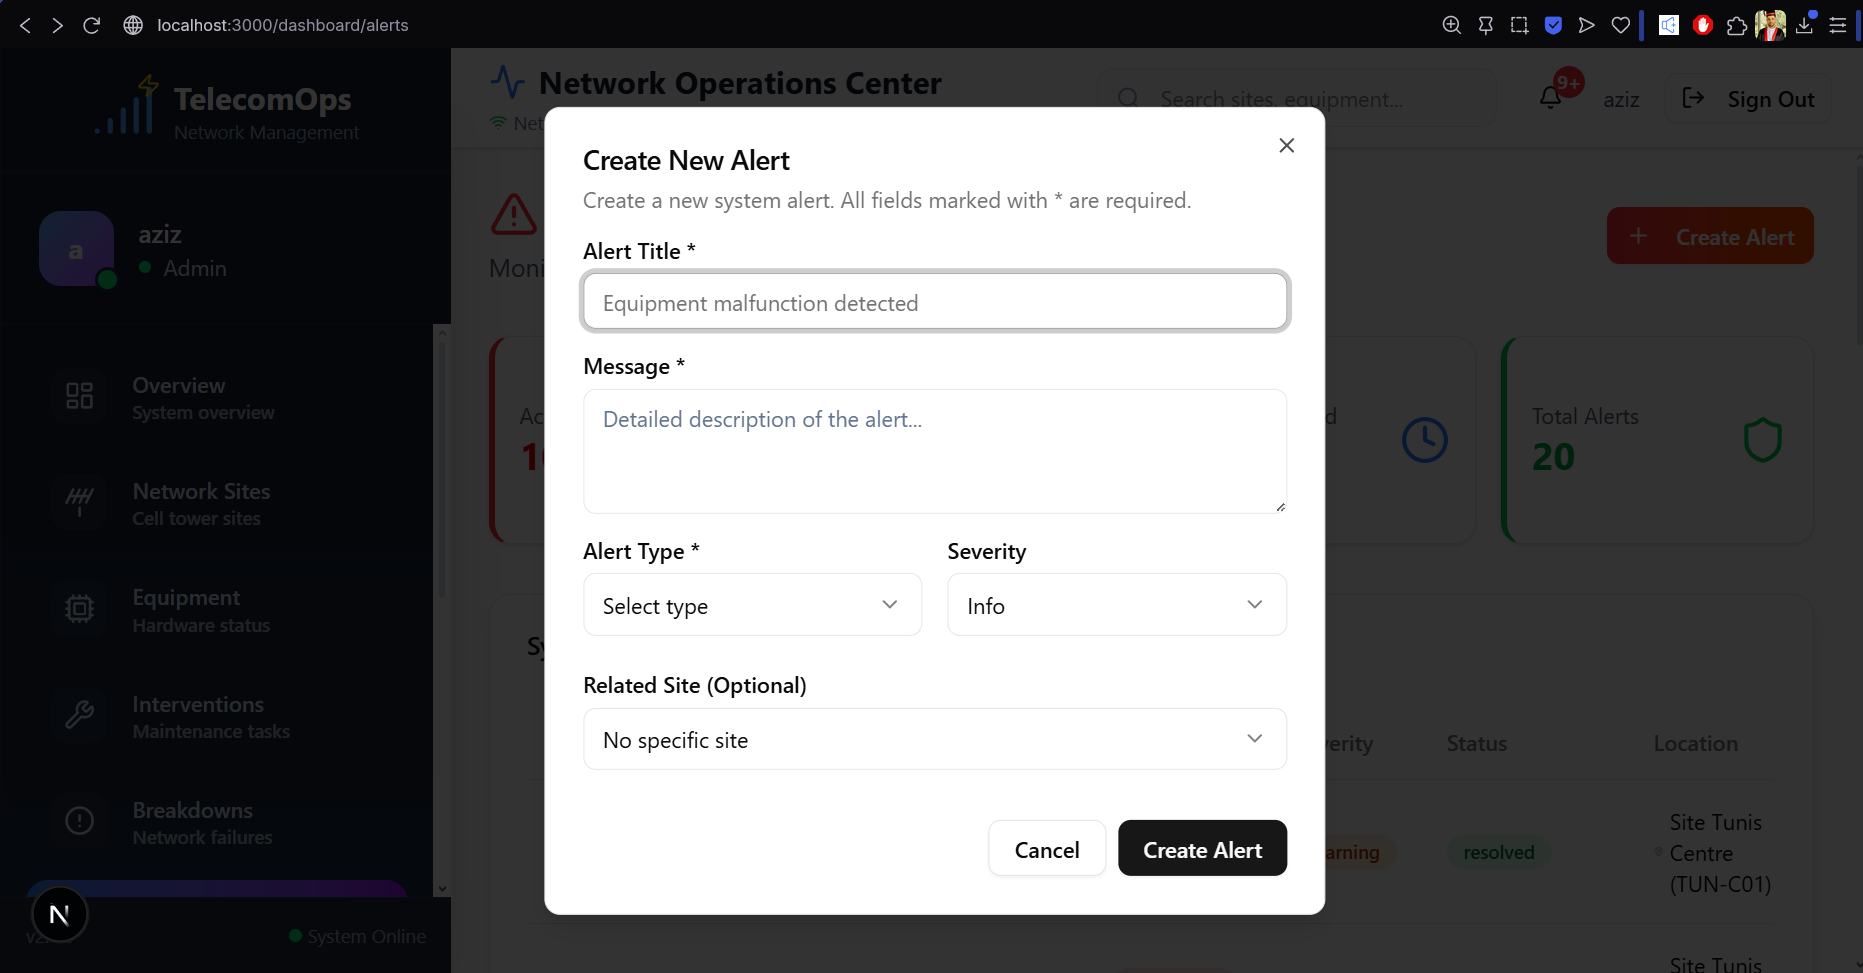
\includegraphics[width=0.95\textwidth]{img/chap_06/screenshot_create_alert.png}}
\caption{Create Alert Dialog}
\end{minipage}
\end{figure}

\begin{figure}[H]
\centering
\begin{minipage}{0.48\textwidth}
\centering
\fbox{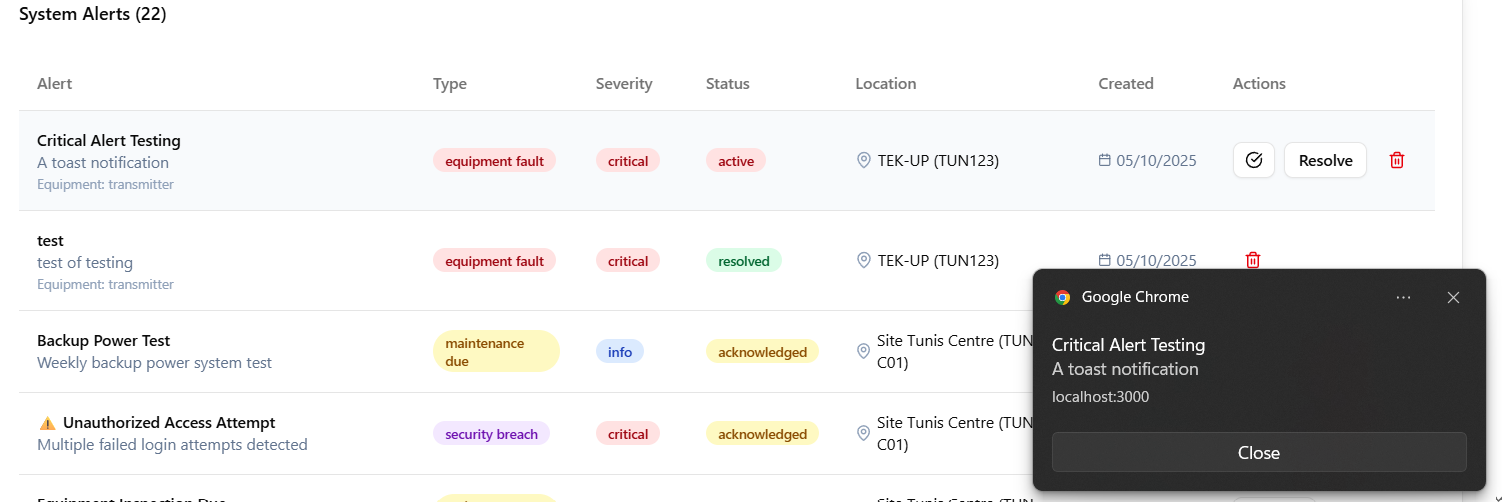
\includegraphics[width=0.95\textwidth]{img/chap_06/screenshot_alert_toast.png}}
\caption{Real-time Notification}
\end{minipage}
\hfill
\begin{minipage}{0.48\textwidth}
\centering
\fbox{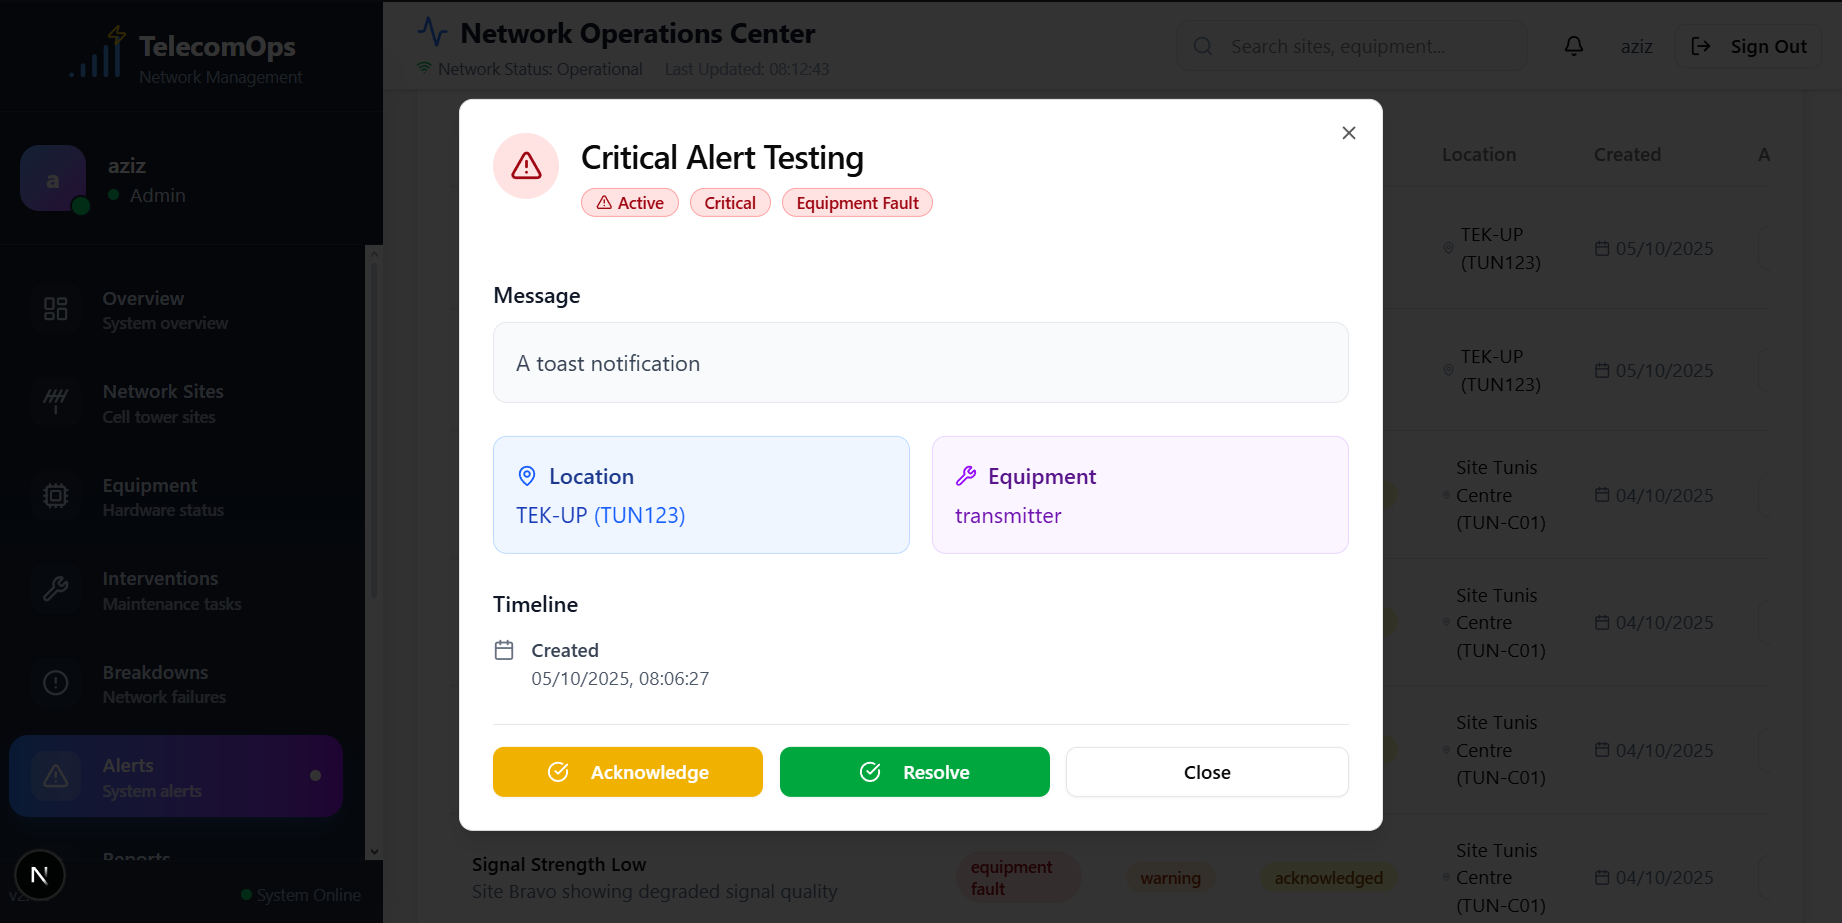
\includegraphics[width=0.95\textwidth]{img/chap_06/screenshot_alert_details.png}}
\caption{Alert Details View}
\end{minipage}
\end{figure}

\begin{figure}[H]
\centering
\begin{minipage}{0.48\textwidth}
\centering
\fbox{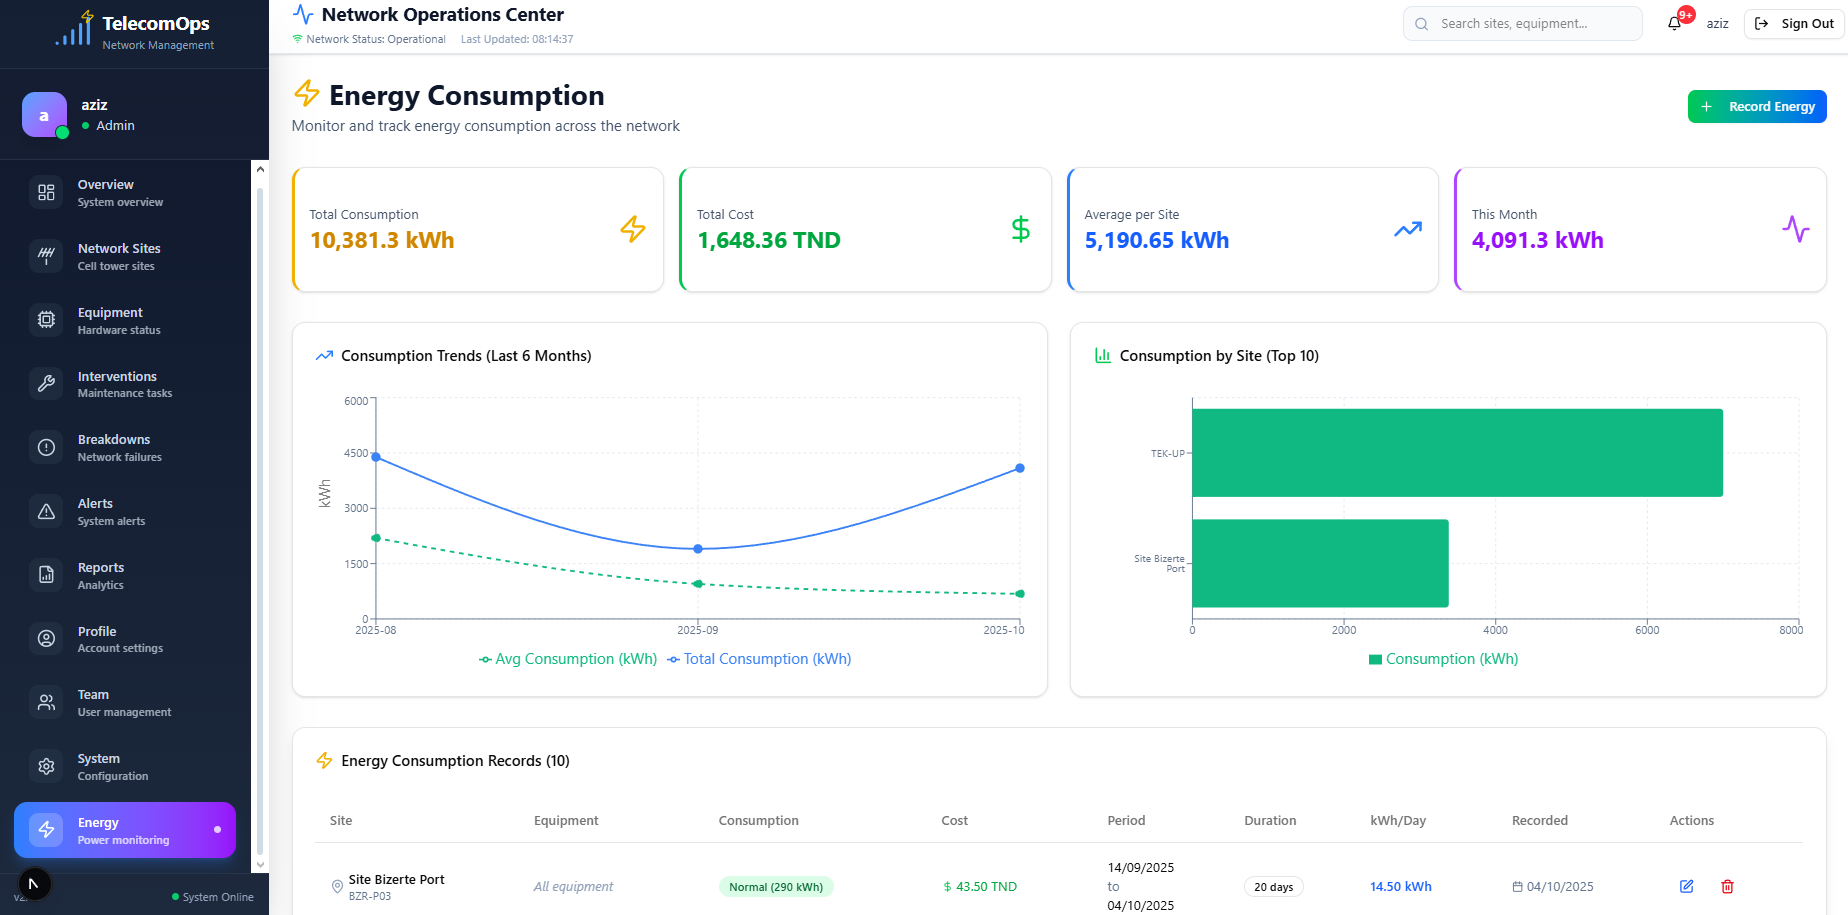
\includegraphics[width=0.95\textwidth]{img/chap_06/screenshot_energy_dashboard.png}}
\caption{Energy Dashboard}
\end{minipage}
\hfill
\begin{minipage}{0.48\textwidth}
\centering
\fbox{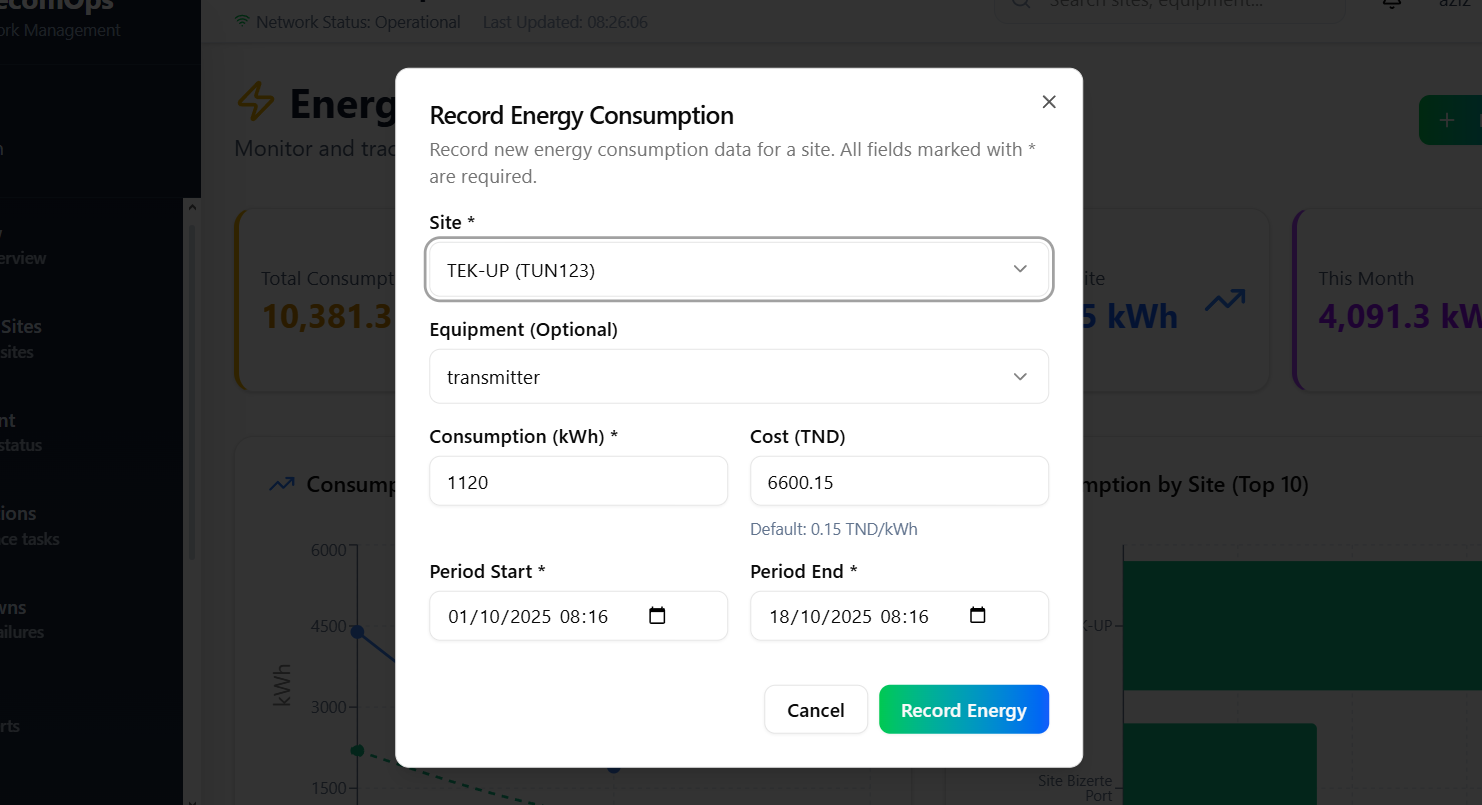
\includegraphics[width=0.95\textwidth]{img/chap_06/screenshot_record_energy.png}}
\caption{Record Energy Dialog}
\end{minipage}
\end{figure}

\begin{figure}[H]
\centering
\begin{minipage}{0.48\textwidth}
\centering
\fbox{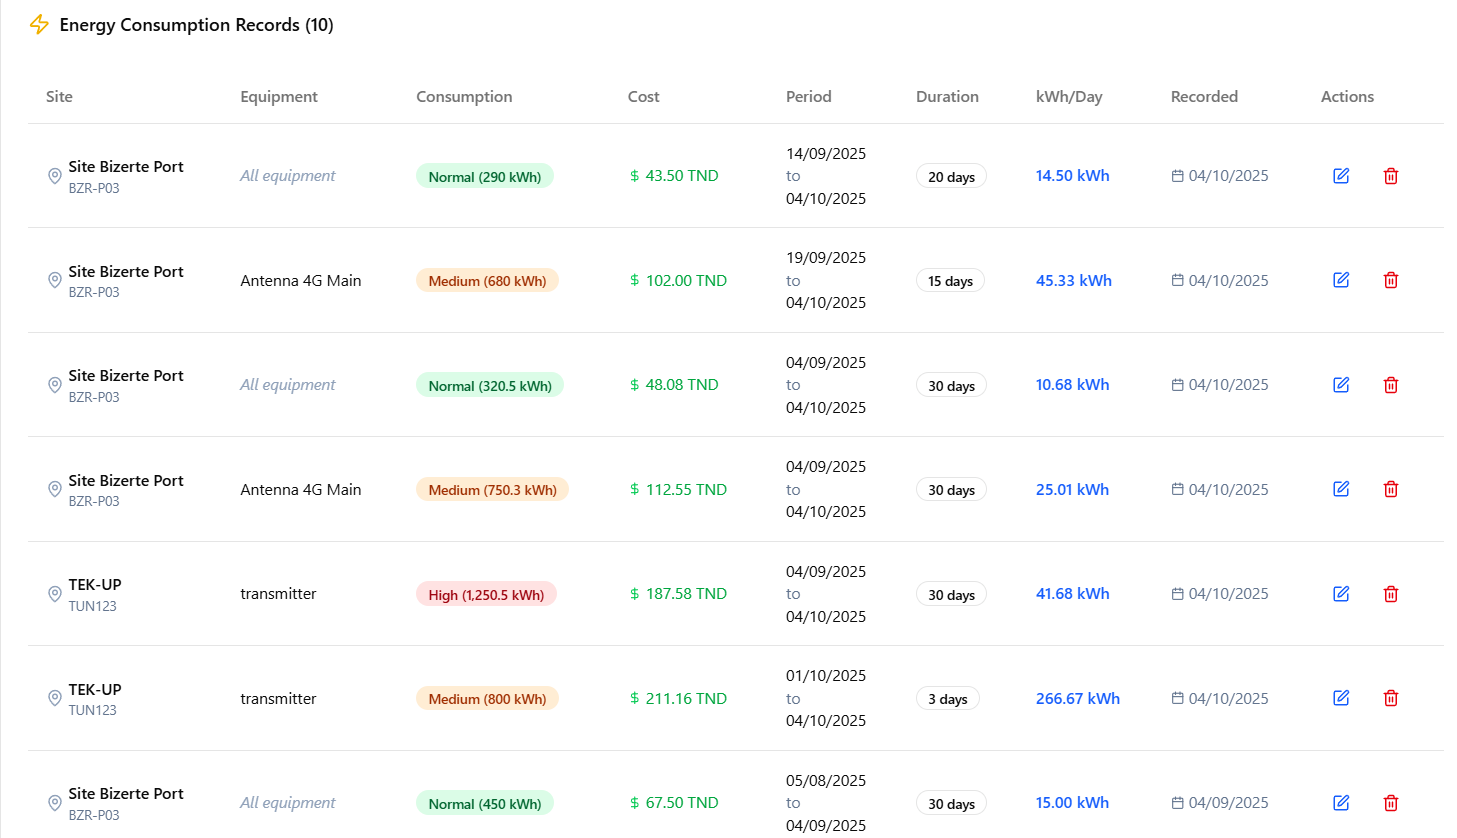
\includegraphics[width=0.95\textwidth]{img/chap_06/screenshot_energy_table.png}}
\caption{Energy Records Table}
\end{minipage}
\hfill
\begin{minipage}{0.48\textwidth}
\centering
\fbox{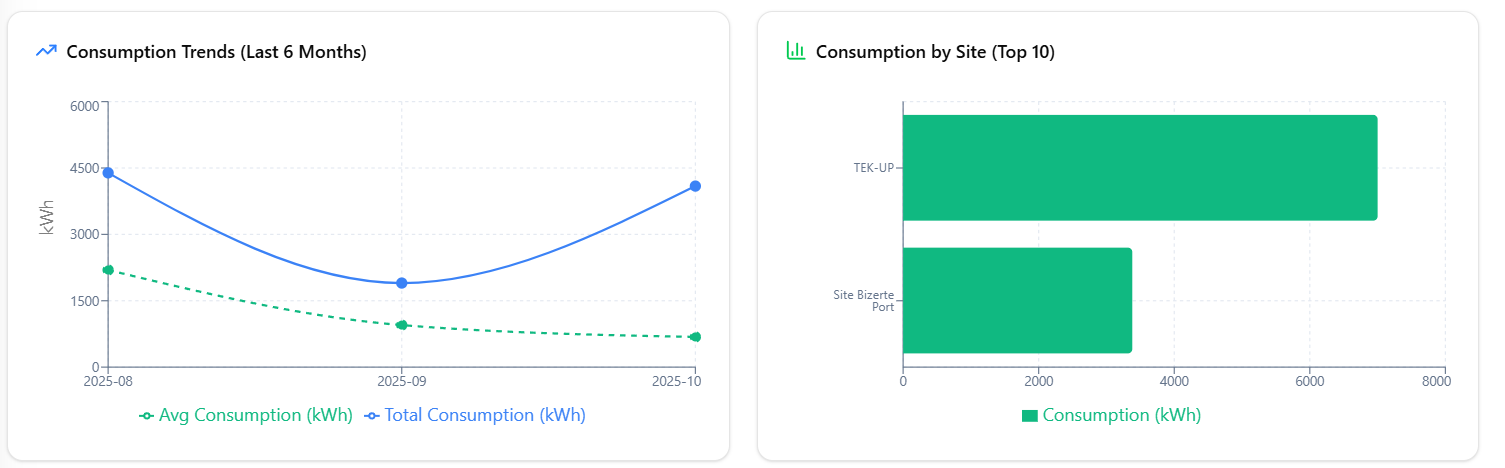
\includegraphics[width=0.95\textwidth]{img/chap_06/screenshot_energy_charts.png}}
\caption{Consumption Charts}
\end{minipage}
\end{figure}

The alerts dashboard displays statistics (active, critical, acknowledged, total) with a comprehensive table showing titles, types, severity, status, and actions. The creation dialog provides validated input for title, message, type, severity, site, and equipment. Real-time toast notifications appear with slide-in animations showing alert details and action buttons. The detail view presents complete information with status-appropriate actions.

The energy dashboard shows statistics (total kWh, cost, average, monthly) with trend charts. The record dialog includes site/equipment selection, kWh input, automatic cost calculation at 0.15 TND/kWh, and period validation. The table displays color-coded consumption (red >1000, orange 500-1000, green <500 kWh), costs, duration, and daily rates. Charts show 6-month trends and top 10 sites comparison.

\section{Technical Challenges and Solutions}

\subsection{Real-time Alert Notifications}

\textbf{Challenge:} Implementing scalable real-time notifications with minimal latency across distributed sessions.

\textbf{Solution:} The system uses Supabase WebSocket subscriptions for bidirectional communication. Critical alerts broadcast events to subscribed clients via the Real-time Engine. The AlertNotificationToast component maintains persistent connections with automatic reconnection logic and exponential backoff. This achieves 200ms delivery latency while supporting concurrent sessions through connection pooling and server-side event filtering.

\subsection{Energy Cost Auto-calculation}

\textbf{Challenge:} Flexible cost calculation supporting automatic rates and manual overrides for varying pricing models.

\textbf{Solution:} The Cost Calculator implements dual-mode calculation: automatic mode multiplies kWh by configured rate (0.15 TND/kWh), manual override allows custom costs. Client-side calculation provides immediate feedback, server-side ensures integrity. The system stores calculated cost and override flag, with centralized rate configuration accessible only to administrators. Historical data remains unchanged when rates update.

\subsection{Consumption Analytics Aggregation}

\textbf{Challenge:} Efficiently aggregating large consumption datasets while providing real-time analytics and optimized rendering.

\textbf{Solution:} PostgreSQL materialized views pre-compute monthly/daily aggregations with incremental refresh. Dashboard queries use views instead of raw records. SQL window functions enable efficient trend calculation. The 6-month chart uses date truncation and GROUP BY, top 10 query employs RANK() with LIMIT. React Query caching stores results with 5-minute TTL. Redis provides sub-100ms response for high-traffic analytics.

\section{Testing and Validation}

\subsection{Functional Testing}

Alert tests validate field validation, type/severity selection, site/equipment association, status transitions, user tracking, and timestamp accuracy. Notification tests verify delivery, toast rendering, auto-dismiss (10s), and manual dismiss. Energy tests validate numeric input, cost calculation accuracy, date validation, and equipment handling. Chart tests confirm data accuracy, aggregation, scaling, and tooltips. Threshold tests verify limit comparison and automatic alert generation.

\subsection{Integration Testing}

Database tests verify Supabase connectivity, Row-Level Security enforcement, foreign key constraints, and transaction integrity. Real-time tests confirm WebSocket establishment, event broadcasting, automatic reconnection, and message ordering. Authentication tests validate role-based access, JWT validation, session management, and unauthorized access prevention. Form tests verify cascading dropdowns, validation consistency, error propagation, and optimistic updates with rollback.

\subsection{Performance Testing}

Alert performance: creation <300ms, notification <200ms, dashboard load <2s (1000+ alerts), 100+ concurrent users. Energy performance: calculation accuracy under load, chart rendering <1s (1000+ points), query <500ms, export optimization. Load tests: 500 concurrent alert creations, 1000 notifications/minute, 10,000 energy queries, 1000 DB ops/second. Memory profiling optimizes heap usage, WebSocket overhead, and React re-renders. Results show linear scaling to 1000 users with under 5 percent degradation.

\section{Conclusion}

Sprint 4 successfully delivers critical systems enhancing TelecomOps capabilities. The Alerts Management System provides incident tracking with sub-200ms real-time notifications via WebSocket architecture, supporting automated/manual creation, role-based workflow, and complete audit trails. The Energy Consumption Monitoring System enables data-driven management with automatic cost calculation, visual analytics, and threshold alerting, processing data efficiently through materialized views with under 1-second dashboard rendering.

Technical achievements include scalable real-time architecture (1000+ sessions), flexible cost calculation with overrides, and high-performance analytics with multi-layered aggregation. Future enhancements will add ML-based anomaly detection, predictive alerting, automated resolution recommendations, comparative site analytics, consumption modeling, and external system integration for advanced operations management and sustainability initiatives.